\documentclass[crop,tikz]{standalone}
\usepackage{physics}
\usetikzlibrary{positioning,3d,decorations.pathreplacing}


\begin{document}
\begin{tikzpicture}
%input
  \begin{scope}[canvas is zy plane at x=-1.8,transform shape]
          \node (source) at (0, 0) {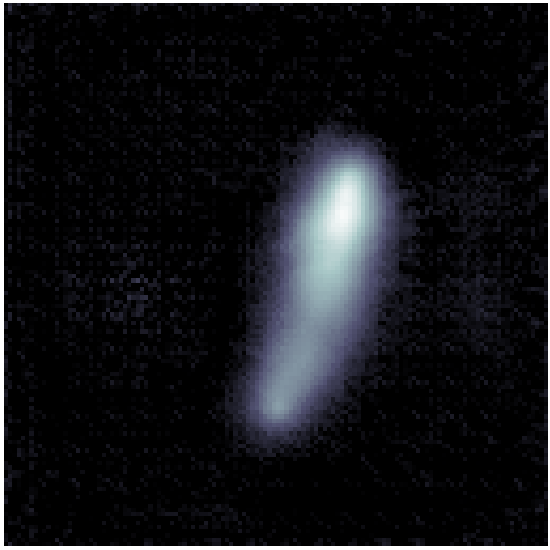
\includegraphics[width=2cm,height=2cm]{source_t2}};
  \end{scope}
  \node[scale=0.6, rotate=40] at (-1.7, 1.4) {$\mathbf{\hat{s}}^{(t)}$};
  \begin{scope}[canvas is zy plane at x=-1.2,transform shape]
	\node{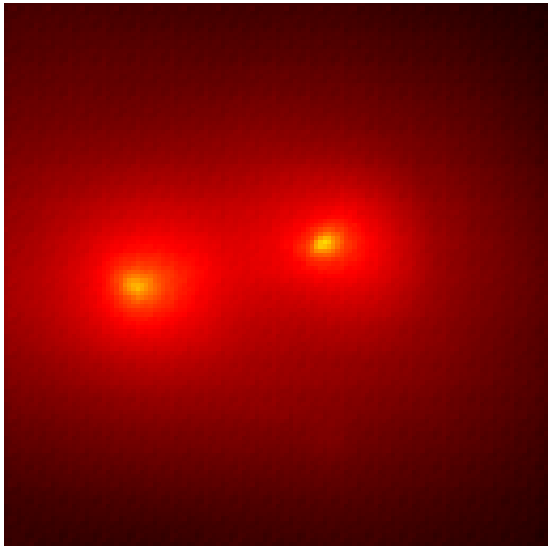
\includegraphics[width=2cm,height=2cm]{kappa_t2}};
  \end{scope}
  \node[scale=0.6, rotate=40] at (-1.1, 1.4) {$\log\boldsymbol{\hat{\kappa}}^{(t)}$};
  \begin{scope}[canvas is yz plane at x=-0.6,transform shape]
    \node{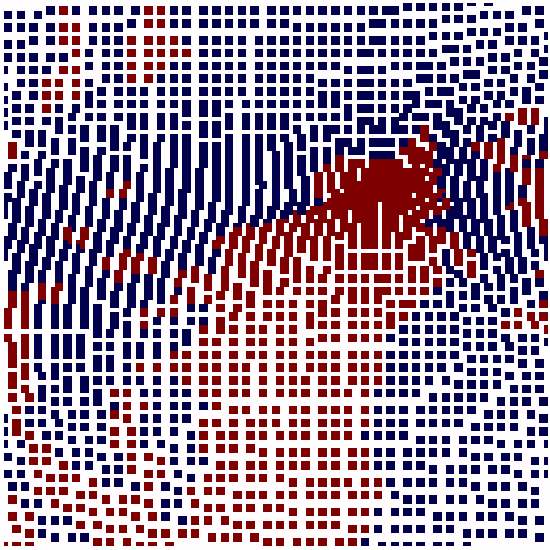
\includegraphics[width=2cm,height=2cm]{source_grad0}};
   %\node[rectangle, minimum size=2cm, fill=black!10, rotate=-90] at (0, 0) {$\grad_{\mathbf{y} \mid \mathbf{\hat{s}^{(t)}}}$};
  \end{scope}
  \node[scale=0.6, rotate=40] at (-0.5, 1.4) {$\grad_{\mathbf{y} \mid \mathbf{\hat{s}^{(t)}}}$};
  \begin{scope}[canvas is yz plane at x=0,transform shape]
    \node{
\includegraphics[width=2cm,height=2cm]{kappa_grad0}};
   %\node[rectangle, minimum size=2cm, fill=black!10, rotate=-90] at (0, 0) {$\grad_{\mathbf{y} \mid \boldsymbol{\hat{\kappa}^{(t)}}}$};
  \end{scope}
  \node[scale=0.6, rotate=40] at (0.15, 1.4) {$\grad_{\mathbf{y} \mid \boldsymbol{\hat{\kappa}^{(t)}}}$};
  \begin{scope}[canvas is zy plane at x=0.6,transform shape]
	\node{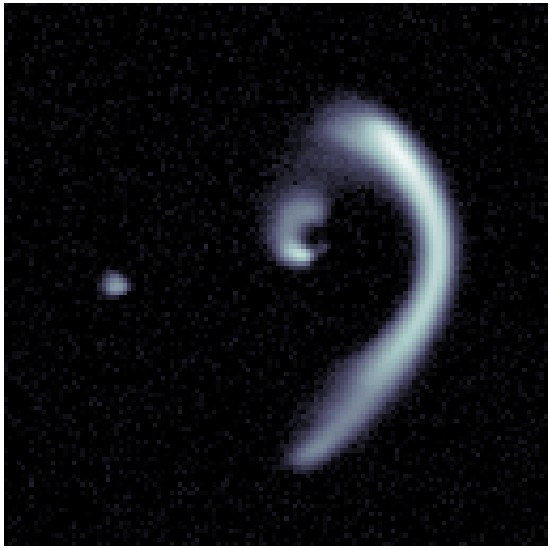
\includegraphics[width=2cm,height=2cm]{lens}};
  \end{scope}
        \node[scale=0.6, rotate=40] at (0.75, 1.4) {$\mathbf{y}$};

\draw[decorate,decoration={brace,amplitude=4pt},xshift=0pt,yshift=0pt,thick,color=darkgray] 
        (-1.9, 1.7) -- (-1., 1.7);
\draw[color=darkgray] (-1.45, 1.85) -- (-1.45, 2.05);
\draw[color=darkgray] (-1.45, 2.05) -- (10, 2.05);
\draw[-latex, color=darkgray] (10, 2.05) -- (10, 0.2);
\draw[-latex, color=darkgray] (0.6, 0) -- (1.5, 0);

% Input layer
\pgfmathsetmacro{\cubex}{0.05}
\pgfmathsetmacro{\cubey}{1.8}
\pgfmathsetmacro{\cubez}{1.8}
\pgfmathsetmacro{\posx}{1}
\pgfmathsetmacro{\posz}{-1.5}
\pgfmathsetmacro{\posy}{0}
\draw[red,fill=pink] (\posx,\posy,\posz) -- ++(-\cubex,0,0) -- ++(0,-\cubey,0) -- ++(\cubex,0,0) -- cycle;
\draw[red,fill=pink] (\posx,\posy,\posz) -- ++(0,0,-\cubez) -- ++(0,-\cubey,0) -- ++(0,0,\cubez) -- cycle;
\draw[red,fill=pink] (\posx,\posy,\posz) -- ++(-\cubex,0,0) -- ++(0,0,-\cubez) -- ++(\cubex,0,0) -- cycle;

\node[xscale=0.4, yscale=0.4, rotate=90] at (1.45, -0.73) { $128 \times 128 \times 128$};

% L11
\pgfmathsetmacro{\cubex}{0.05}
\pgfmathsetmacro{\cubey}{1.8}
\pgfmathsetmacro{\cubez}{1.8}
\pgfmathsetmacro{\posx}{1.2}
\pgfmathsetmacro{\posz}{-1.5}
\pgfmathsetmacro{\posy}{0}
\draw[darkgray,fill=gray] (\posx,\posy,\posz) -- ++(-\cubex,0,0) -- ++(0,-\cubey,0) -- ++(\cubex,0,0) -- cycle;
\draw[darkgray,fill=gray] (\posx,\posy,\posz) -- ++(0,0,-\cubez) -- ++(0,-\cubey,0) -- ++(0,0,\cubez) -- cycle;
\draw[darkgray,fill=gray] (\posx,\posy,\posz) -- ++(-\cubex,0,0) -- ++(0,0,-\cubez) -- ++(\cubex,0,0) -- cycle;


% L12
\pgfmathsetmacro{\cubex}{0.05}
\pgfmathsetmacro{\cubey}{1.8}
\pgfmathsetmacro{\cubez}{1.8}
\pgfmathsetmacro{\posx}{1.4}
\pgfmathsetmacro{\posz}{-1.5}
\pgfmathsetmacro{\posy}{0}
\draw[darkgray,fill=gray] (\posx,\posy,\posz) -- ++(-\cubex,0,0) -- ++(0,-\cubey,0) -- ++(\cubex,0,0) -- cycle;
\draw[darkgray,fill=gray] (\posx,\posy,\posz) -- ++(0,0,-\cubez) -- ++(0,-\cubey,0) -- ++(0,0,\cubez) -- cycle;
\draw[darkgray,fill=gray] (\posx,\posy,\posz) -- ++(-\cubex,0,0) -- ++(0,0,-\cubez) -- ++(\cubex,0,0) -- cycle;

% Skip 1
\draw[-latex, color=darkgray] (1.4, -0.9, -2.4) -- (3.7, -0.9, -2.4);
%\node[xscale=0.4, yscale=0.4] at (3.5,0.1) {Skip connection};
\node[rectangle, rounded corners, draw=black, fill=black!20, xscale=0.4, yscale=0.4, 
        minimum height=1cm, minimum width=2cm] (gru1) at (5.02, 0.03) {GRU};
\draw[-latex, color=darkgray] (4.5, -0.9, -2.4) -- (7.18, -0.9, -2.4);

%\draw[-latex, thick] (1.4, -0.9, -2.4) -- (4, -0.9, -2.4); % adjust with G bar


% L13
\pgfmathsetmacro{\cubex}{0.075}
\pgfmathsetmacro{\cubey}{0.9}
\pgfmathsetmacro{\cubez}{0.9}
\pgfmathsetmacro{\posx}{1.4}
\pgfmathsetmacro{\posz}{-1.5}
\pgfmathsetmacro{\posy}{-2.}
\draw[blue,fill=cyan] (\posx,\posy,\posz) -- ++(-\cubex,0,0) -- ++(0,-\cubey,0) -- ++(\cubex,0,0) -- cycle;
\draw[blue,fill=cyan] (\posx,\posy,\posz) -- ++(0,0,-\cubez) -- ++(0,-\cubey,0) -- ++(0,0,\cubez) -- cycle;
\draw[blue,fill=cyan] (\posx,\posy,\posz) -- ++(-\cubex,0,0) -- ++(0,0,-\cubez) -- ++(\cubex,0,0) -- cycle;

% downsample 1
\draw[-latex, color=blue] (1.38, -1.8, -1.5) -- (1.38, -2, -1.5);

\node[xscale=0.4, yscale=0.4, rotate=90] at (1.83, -1.9) { $64 \times 64 \times 256$};

% L21 
\pgfmathsetmacro{\cubex}{0.075}
\pgfmathsetmacro{\cubey}{0.9}
\pgfmathsetmacro{\cubez}{0.9}
\pgfmathsetmacro{\posx}{1.6}
\pgfmathsetmacro{\posz}{-1.5}
\pgfmathsetmacro{\posy}{-2.}
\draw[darkgray,fill=gray] (\posx,\posy,\posz) -- ++(-\cubex,0,0) -- ++(0,-\cubey,0) -- ++(\cubex,0,0) -- cycle;
\draw[darkgray,fill=gray] (\posx,\posy,\posz) -- ++(0,0,-\cubez) -- ++(0,-\cubey,0) -- ++(0,0,\cubez) -- cycle;
\draw[darkgray,fill=gray] (\posx,\posy,\posz) -- ++(-\cubex,0,0) -- ++(0,0,-\cubez) -- ++(\cubex,0,0) -- cycle;


% L22
\pgfmathsetmacro{\cubex}{0.075}
\pgfmathsetmacro{\cubey}{0.9}
\pgfmathsetmacro{\cubez}{0.9}
\pgfmathsetmacro{\posx}{1.8}
\pgfmathsetmacro{\posz}{-1.5}
\pgfmathsetmacro{\posy}{-2.}
\draw[darkgray,fill=gray] (\posx,\posy,\posz) -- ++(-\cubex,0,0) -- ++(0,-\cubey,0) -- ++(\cubex,0,0) -- cycle;
\draw[darkgray,fill=gray] (\posx,\posy,\posz) -- ++(0,0,-\cubez) -- ++(0,-\cubey,0) -- ++(0,0,\cubez) -- cycle;
\draw[darkgray,fill=gray] (\posx,\posy,\posz) -- ++(-\cubex,0,0) -- ++(0,0,-\cubez) -- ++(\cubex,0,0) -- cycle;

% Skip 2
\draw[-latex, color=darkgray] (1.8, -2.45, -1.95) -- (3.88, -2.45, -1.95);
\node[rectangle, rounded corners, draw=black, fill=black!20, xscale=0.4, yscale=0.4, 
        minimum height=1cm, minimum width=2cm] (gru1) at (5.02, -1.7) {GRU};
\draw[-latex, color=darkgray] (4.66, -2.45, -1.95) -- (6.9, -2.45, -1.95);
%\draw[-latex, thick] (1.8, -2.45, -1.95) -- (4.19, -2.45, -1.95);

% L23
\pgfmathsetmacro{\cubex}{0.125}
\pgfmathsetmacro{\cubey}{0.45}
\pgfmathsetmacro{\cubez}{0.45}
\pgfmathsetmacro{\posx}{1.8}
\pgfmathsetmacro{\posz}{-1.5}
\pgfmathsetmacro{\posy}{-3.1}
\draw[blue,fill=cyan] (\posx,\posy,\posz) -- ++(-\cubex,0,0) -- ++(0,-\cubey,0) -- ++(\cubex,0,0) -- cycle;
\draw[blue,fill=cyan] (\posx,\posy,\posz) -- ++(0,0,-\cubez) -- ++(0,-\cubey,0) -- ++(0,0,\cubez) -- cycle;
\draw[blue,fill=cyan] (\posx,\posy,\posz) -- ++(-\cubex,0,0) -- ++(0,0,-\cubez) -- ++(\cubex,0,0) -- cycle;

% downsample 2
\draw[-latex, color=blue] (1.76, -2.9, -1.5) -- (1.76, -3.1, -1.5);

\node[xscale=0.4, yscale=0.4] at (1.9, -2.7) { $32^2 \times 512$};
%\node[xscale=0.4, yscale=0.4, rotate=90] at (2.15, -2.7) { $32^2 \times 512$};

% L31
\pgfmathsetmacro{\cubex}{0.125}
\pgfmathsetmacro{\cubey}{0.45}
\pgfmathsetmacro{\cubez}{0.45}
\pgfmathsetmacro{\posx}{2.}
\pgfmathsetmacro{\posz}{-1.5}
\pgfmathsetmacro{\posy}{-3.1}
\draw[darkgray,fill=gray] (\posx,\posy,\posz) -- ++(-\cubex,0,0) -- ++(0,-\cubey,0) -- ++(\cubex,0,0) -- cycle;
\draw[darkgray,fill=gray] (\posx,\posy,\posz) -- ++(0,0,-\cubez) -- ++(0,-\cubey,0) -- ++(0,0,\cubez) -- cycle;
\draw[darkgray,fill=gray] (\posx,\posy,\posz) -- ++(-\cubex,0,0) -- ++(0,0,-\cubez) -- ++(\cubex,0,0) -- cycle;

% L32
\pgfmathsetmacro{\cubex}{0.125}
\pgfmathsetmacro{\cubey}{0.45}
\pgfmathsetmacro{\cubez}{0.45}
\pgfmathsetmacro{\posx}{2.2}
\pgfmathsetmacro{\posz}{-1.5}
\pgfmathsetmacro{\posy}{-3.1}
\draw[darkgray,fill=gray] (\posx,\posy,\posz) -- ++(-\cubex,0,0) -- ++(0,-\cubey,0) -- ++(\cubex,0,0) -- cycle;
\draw[darkgray,fill=gray] (\posx,\posy,\posz) -- ++(0,0,-\cubez) -- ++(0,-\cubey,0) -- ++(0,0,\cubez) -- cycle;
\draw[darkgray,fill=gray] (\posx,\posy,\posz) -- ++(-\cubex,0,0) -- ++(0,0,-\cubez) -- ++(\cubex,0,0) -- cycle;

% Skip 3
\draw[-latex, color=darkgray] (2.2, -3.325, -1.725) -- (3.97, -3.325, -1.725);
\node[rectangle, rounded corners, draw=black, fill=black!20, xscale=0.4, yscale=0.4, 
        minimum height=1cm, minimum width=2cm] (gru1) at (5.02,-2.66) {GRU};
\draw[-latex, color=darkgray] (4.76, -3.325, -1.725) -- (6.5, -3.325, -1.725);
%\draw[-latex, thick] (2.2, -3.325, -1.725) -- (4.27, -3.325, -1.725); % adjust with the middle g bar

% L33
\pgfmathsetmacro{\cubex}{0.25}
\pgfmathsetmacro{\cubey}{0.2}
\pgfmathsetmacro{\cubez}{0.2}
\pgfmathsetmacro{\posx}{2.2}
\pgfmathsetmacro{\posz}{-1.5}
\pgfmathsetmacro{\posy}{-3.8}
\draw[blue,fill=cyan] (\posx,\posy,\posz) -- ++(-\cubex,0,0) -- ++(0,-\cubey,0) -- ++(\cubex,0,0) -- cycle;
\draw[blue,fill=cyan] (\posx,\posy,\posz) -- ++(0,0,-\cubez) -- ++(0,-\cubey,0) -- ++(0,0,\cubez) -- cycle;
\draw[blue,fill=cyan] (\posx,\posy,\posz) -- ++(-\cubex,0,0) -- ++(0,0,-\cubez) -- ++(\cubex,0,0) -- cycle;

% downsample 3
\draw[-latex, color=blue] (2.15, -3.55, -1.5) -- (2.15, -3.8, -1.5);

\node[xscale=0.4, yscale=0.4] at (2.15, -3.3) { $16^2 \times 1024$};

% L41
\pgfmathsetmacro{\cubex}{0.25}
\pgfmathsetmacro{\cubey}{0.2}
\pgfmathsetmacro{\cubez}{0.2}
\pgfmathsetmacro{\posx}{2.5}
\pgfmathsetmacro{\posz}{-1.5}
\pgfmathsetmacro{\posy}{-3.8}
\draw[darkgray,fill=gray] (\posx,\posy,\posz) -- ++(-\cubex,0,0) -- ++(0,-\cubey,0) -- ++(\cubex,0,0) -- cycle;
\draw[darkgray,fill=gray] (\posx,\posy,\posz) -- ++(0,0,-\cubez) -- ++(0,-\cubey,0) -- ++(0,0,\cubez) -- cycle;
\draw[darkgray,fill=gray] (\posx,\posy,\posz) -- ++(-\cubex,0,0) -- ++(0,0,-\cubez) -- ++(\cubex,0,0) -- cycle;

% L42
\pgfmathsetmacro{\cubex}{0.25}
\pgfmathsetmacro{\cubey}{0.2}
\pgfmathsetmacro{\cubez}{0.2}
\pgfmathsetmacro{\posx}{2.8}
\pgfmathsetmacro{\posz}{-1.5}
\pgfmathsetmacro{\posy}{-3.8}
\draw[darkgray,fill=gray] (\posx,\posy,\posz) -- ++(-\cubex,0,0) -- ++(0,-\cubey,0) -- ++(\cubex,0,0) -- cycle;
\draw[darkgray,fill=gray] (\posx,\posy,\posz) -- ++(0,0,-\cubez) -- ++(0,-\cubey,0) -- ++(0,0,\cubez) -- cycle;
\draw[darkgray,fill=gray] (\posx,\posy,\posz) -- ++(-\cubex,0,0) -- ++(0,0,-\cubez) -- ++(\cubex,0,0) -- cycle;

% Skip 4
\draw[-latex, color=darkgray] (2.8, -3.9, -1.6) -- (4.01, -3.9, -1.6);
\node[rectangle, rounded corners, draw=black, fill=black!20, xscale=0.4, yscale=0.4, 
        minimum height=1cm, minimum width=2cm] (gru1) at (5.02,-3.27) {GRU};
\draw[-latex, color=darkgray] (4.8, -3.9, -1.6) -- (5.7, -3.9, -1.6);
%\node[scale=0.6] at (6.15, -3.29) {$\boldsymbol{\oplus}$};
%\draw[-latex, thick] (2.8, -3.9, -1.6) -- (4.3, -3.9, -1.6); % adjust with the middle g bar


% L43
\pgfmathsetmacro{\cubex}{0.25}
\pgfmathsetmacro{\cubey}{0.1}
\pgfmathsetmacro{\cubez}{0.1}
\pgfmathsetmacro{\posx}{2.8}
\pgfmathsetmacro{\posz}{-1.5}
\pgfmathsetmacro{\posy}{-4.35}
\draw[blue,fill=cyan] (\posx,\posy,\posz) -- ++(-\cubex,0,0) -- ++(0,-\cubey,0) -- ++(\cubex,0,0) -- cycle;
\draw[blue,fill=cyan] (\posx,\posy,\posz) -- ++(0,0,-\cubez) -- ++(0,-\cubey,0) -- ++(0,0,\cubez) -- cycle;
\draw[blue,fill=cyan] (\posx,\posy,\posz) -- ++(-\cubex,0,0) -- ++(0,0,-\cubez) -- ++(\cubex,0,0) -- cycle;

% downsample 4
\draw[-latex, color=blue] (2.7, -4, -1.5) -- (2.7, -4.35, -1.5);

\node[xscale=0.4, yscale=0.4] at (2.8, -3.8) { $8^2 \times 1024$};

% L51
\pgfmathsetmacro{\cubex}{0.25}
\pgfmathsetmacro{\cubey}{0.1}
\pgfmathsetmacro{\cubez}{0.1}
\pgfmathsetmacro{\posx}{3.1}
\pgfmathsetmacro{\posz}{-1.5}
\pgfmathsetmacro{\posy}{-4.35}
\draw[darkgray,fill=gray] (\posx,\posy,\posz) -- ++(-\cubex,0,0) -- ++(0,-\cubey,0) -- ++(\cubex,0,0) -- cycle;
\draw[darkgray,fill=gray] (\posx,\posy,\posz) -- ++(0,0,-\cubez) -- ++(0,-\cubey,0) -- ++(0,0,\cubez) -- cycle;
\draw[darkgray,fill=gray] (\posx,\posy,\posz) -- ++(-\cubex,0,0) -- ++(0,0,-\cubez) -- ++(\cubex,0,0) -- cycle;


% L52
\pgfmathsetmacro{\cubex}{0.25}
\pgfmathsetmacro{\cubey}{0.1}
\pgfmathsetmacro{\cubez}{0.1}
\pgfmathsetmacro{\posx}{3.4}
\pgfmathsetmacro{\posz}{-1.5}
\pgfmathsetmacro{\posy}{-4.35}
\draw[darkgray,fill=gray] (\posx,\posy,\posz) -- ++(-\cubex,0,0) -- ++(0,-\cubey,0) -- ++(\cubex,0,0) -- cycle;
\draw[darkgray,fill=gray] (\posx,\posy,\posz) -- ++(0,0,-\cubez) -- ++(0,-\cubey,0) -- ++(0,0,\cubez) -- cycle;
\draw[darkgray,fill=gray] (\posx,\posy,\posz) -- ++(-\cubex,0,0) -- ++(0,0,-\cubez) -- ++(\cubex,0,0) -- cycle;


% Skip 4
\draw[-latex, color=darkgray] (3.4, -4.4, -1.55) -- (4.02, -4.4, -1.55);
\node[rectangle, rounded corners, draw=black, fill=black!20, xscale=0.4, yscale=0.4, 
        minimum height=1cm, minimum width=2cm] (gru1) at (5.02,-3.8) {GRU};
%\draw[-latex, color=darkgray] (4.82, -4.4, -1.55) -- (5.69, % Skip 4
\draw[-latex, color=darkgray] (3.4, -4.4, -1.55) -- (4.02, -4.4, -1.55);
\node[rectangle, rounded corners, draw=black, fill=black!20, xscale=0.4, yscale=0.4, 
        minimum height=1cm, minimum width=2cm] (gru1) at (5.02,-3.8) {GRU};
\draw[-latex, color=darkgray] (4.82, -4.4, -1.55) -- (5.12, -4.4, -1.55);
%\draw[-latex, thick] (3.4, -4.4, -1.55) -- (4.3, -4.4, -1.55); % adjust with the middle g bar

% L53
\pgfmathsetmacro{\cubex}{0.25}
\pgfmathsetmacro{\cubey}{0.05}
\pgfmathsetmacro{\cubez}{0.05}
\pgfmathsetmacro{\posx}{3.4}
\pgfmathsetmacro{\posz}{-1.5}
\pgfmathsetmacro{\posy}{-4.875}
\draw[blue,fill=cyan] (\posx,\posy,\posz) -- ++(-\cubex,0,0) -- ++(0,-\cubey,0) -- ++(\cubex,0,0) -- cycle;
\draw[blue,fill=cyan] (\posx,\posy,\posz) -- ++(0,0,-\cubez) -- ++(0,-\cubey,0) -- ++(0,0,\cubez) -- cycle;
\draw[blue,fill=cyan] (\posx,\posy,\posz) -- ++(-\cubex,0,0) -- ++(0,0,-\cubez) -- ++(\cubex,0,0) -- cycle;

% downsample 4
\draw[-latex, color=blue] (3.3, -4.45, -1.5) -- (3.3, -4.875, -1.5);

\node[xscale=0.4, yscale=0.4] at (3.4, -4.3) { $4^2 \times 1024$};

% Bottleneck
\draw[-latex, color=darkgray] (3.4, -4.9, -1.525) -- (4.02, -4.9, -1.525);
\node[rectangle, rounded corners, draw=black, fill=black!20, xscale=0.4, yscale=0.4, 
        minimum height=1cm, minimum width=2cm] (gru1) at (5.02,-4.3) {GRU};
\draw[-latex, color=darkgray] (4.82, -4.9, -1.525) -- (5.4, -4.9, -1.525);
%\draw[-latex, thick] (3.4, -4.9, -1.55) -- (4.3, -4.9, -1.55); % adjust with the middle g bar


% UB
\pgfmathsetmacro{\cubex}{0.25}
\pgfmathsetmacro{\cubey}{0.05}
\pgfmathsetmacro{\cubez}{0.05}
\pgfmathsetmacro{\posx}{5.65}
\pgfmathsetmacro{\posz}{-1.5}
\pgfmathsetmacro{\posy}{-4.875}
\draw[brown,fill=orange] (\posx,\posy,\posz) -- ++(-\cubex,0,0) -- ++(0,-\cubey,0) -- ++(\cubex,0,0) -- cycle;
\draw[brown,fill=orange] (\posx,\posy,\posz) -- ++(0,0,-\cubez) -- ++(0,-\cubey,0) -- ++(0,0,\cubez) -- cycle;
\draw[brown,fill=orange] (\posx,\posy,\posz) -- ++(-\cubex,0,0) -- ++(0,0,-\cubez) -- ++(\cubex,0,0) -- cycle;

\draw[-latex, color=brown] (5.5,-4.9,-1.525) -- (5.5,-4.45,-1.525);


% U511
\pgfmathsetmacro{\cubex}{0.25}
\pgfmathsetmacro{\cubey}{0.1}
\pgfmathsetmacro{\cubez}{0.1}
\pgfmathsetmacro{\posx}{5.4}
\pgfmathsetmacro{\posz}{-1.5}
\pgfmathsetmacro{\posy}{-4.35}
\draw[darkgray,fill=white] (\posx,\posy,\posz) -- ++(-\cubex,0,0) -- ++(0,-\cubey,0) -- ++(\cubex,0,0) -- cycle;
\draw[darkgray,fill=white] (\posx,\posy,\posz) -- ++(0,0,-\cubez) -- ++(0,-\cubey,0) -- ++(0,0,\cubez) -- cycle;
\draw[darkgray,fill=white] (\posx,\posy,\posz) -- ++(-\cubex,0,0) -- ++(0,0,-\cubez) -- ++(\cubex,0,0) -- cycle;

% U512
\pgfmathsetmacro{\cubex}{0.25}
\pgfmathsetmacro{\cubey}{0.1}
\pgfmathsetmacro{\cubez}{0.1}
\pgfmathsetmacro{\posx}{5.65}
\pgfmathsetmacro{\posz}{-1.5}
\pgfmathsetmacro{\posy}{-4.35}
\draw[darkgray,fill=gray] (\posx,\posy,\posz) -- ++(-\cubex,0,0) -- ++(0,-\cubey,0) -- ++(\cubex,0,0) -- cycle;
\draw[darkgray,fill=gray] (\posx,\posy,\posz) -- ++(0,0,-\cubez) -- ++(0,-\cubey,0) -- ++(0,0,\cubez) -- cycle;
\draw[darkgray,fill=gray] (\posx,\posy,\posz) -- ++(-\cubex,0,0) -- ++(0,0,-\cubez) -- ++(\cubex,0,0) -- cycle;

% U52
\pgfmathsetmacro{\cubex}{0.25}
\pgfmathsetmacro{\cubey}{0.1}
\pgfmathsetmacro{\cubez}{0.1}
\pgfmathsetmacro{\posx}{5.95}
\pgfmathsetmacro{\posz}{-1.5}
\pgfmathsetmacro{\posy}{-4.35}
\draw[darkgray,fill=gray] (\posx,\posy,\posz) -- ++(-\cubex,0,0) -- ++(0,-\cubey,0) -- ++(\cubex,0,0) -- cycle;
\draw[darkgray,fill=gray] (\posx,\posy,\posz) -- ++(0,0,-\cubez) -- ++(0,-\cubey,0) -- ++(0,0,\cubez) -- cycle;
\draw[darkgray,fill=gray] (\posx,\posy,\posz) -- ++(-\cubex,0,0) -- ++(0,0,-\cubez) -- ++(\cubex,0,0) -- cycle;

 %U53
\pgfmathsetmacro{\cubex}{0.25}
\pgfmathsetmacro{\cubey}{0.1}
\pgfmathsetmacro{\cubez}{0.1}
\pgfmathsetmacro{\posx}{6.25}
\pgfmathsetmacro{\posz}{-1.5}
\pgfmathsetmacro{\posy}{-4.35}
\draw[brown,fill=orange] (\posx,\posy,\posz) -- ++(-\cubex,0,0) -- ++(0,-\cubey,0) -- ++(\cubex,0,0) -- cycle;
\draw[brown,fill=orange] (\posx,\posy,\posz) -- ++(0,0,-\cubez) -- ++(0,-\cubey,0) -- ++(0,0,\cubez) -- cycle;
\draw[brown,fill=orange] (\posx,\posy,\posz) -- ++(-\cubex,0,0) -- ++(0,0,-\cubez) -- ++(\cubex,0,0) -- cycle;

\draw[-latex, color=brown] (6.1, -4.35, -1.55) -- (6.1, -4, -1.55);

% U421
\pgfmathsetmacro{\cubex}{0.25}
\pgfmathsetmacro{\cubey}{0.2}
\pgfmathsetmacro{\cubez}{0.2}
\pgfmathsetmacro{\posx}{6}
\pgfmathsetmacro{\posz}{-1.5}
\pgfmathsetmacro{\posy}{-3.8}
\draw[darkgray,fill=white] (\posx,\posy,\posz) -- ++(-\cubex,0,0) -- ++(0,-\cubey,0) -- ++(\cubex,0,0) -- cycle;
\draw[darkgray,fill=white] (\posx,\posy,\posz) -- ++(0,0,-\cubez) -- ++(0,-\cubey,0) -- ++(0,0,\cubez) -- cycle;
\draw[darkgray,fill=white] (\posx,\posy,\posz) -- ++(-\cubex,0,0) -- ++(0,0,-\cubez) -- ++(\cubex,0,0) -- cycle;


% U522
\pgfmathsetmacro{\cubex}{0.25}
\pgfmathsetmacro{\cubey}{0.2}
\pgfmathsetmacro{\cubez}{0.2}
\pgfmathsetmacro{\posx}{6.25}
\pgfmathsetmacro{\posz}{-1.5}
\pgfmathsetmacro{\posy}{-3.8}
\draw[darkgray,fill=gray] (\posx,\posy,\posz) -- ++(-\cubex,0,0) -- ++(0,-\cubey,0) -- ++(\cubex,0,0) -- cycle;
\draw[darkgray,fill=gray] (\posx,\posy,\posz) -- ++(0,0,-\cubez) -- ++(0,-\cubey,0) -- ++(0,0,\cubez) -- cycle;
\draw[darkgray,fill=gray] (\posx,\posy,\posz) -- ++(-\cubex,0,0) -- ++(0,0,-\cubez) -- ++(\cubex,0,0) -- cycle;

% U53
\pgfmathsetmacro{\cubex}{0.25}
\pgfmathsetmacro{\cubey}{0.2}
\pgfmathsetmacro{\cubez}{0.2}
\pgfmathsetmacro{\posx}{6.55}
\pgfmathsetmacro{\posz}{-1.5}
\pgfmathsetmacro{\posy}{-3.8}
\draw[darkgray,fill=gray] (\posx,\posy,\posz) -- ++(-\cubex,0,0) -- ++(0,-\cubey,0) -- ++(\cubex,0,0) -- cycle;
\draw[darkgray,fill=gray] (\posx,\posy,\posz) -- ++(0,0,-\cubez) -- ++(0,-\cubey,0) -- ++(0,0,\cubez) -- cycle;
\draw[darkgray,fill=gray] (\posx,\posy,\posz) -- ++(-\cubex,0,0) -- ++(0,0,-\cubez) -- ++(\cubex,0,0) -- cycle;

% U54
\pgfmathsetmacro{\cubex}{0.25}
\pgfmathsetmacro{\cubey}{0.2}
\pgfmathsetmacro{\cubez}{0.2}
\pgfmathsetmacro{\posx}{6.85}
\pgfmathsetmacro{\posz}{-1.5}
\pgfmathsetmacro{\posy}{-3.8}
\draw[brown,fill=orange] (\posx,\posy,\posz) -- ++(-\cubex,0,0) -- ++(0,-\cubey,0) -- ++(\cubex,0,0) -- cycle;
\draw[brown,fill=orange] (\posx,\posy,\posz) -- ++(0,0,-\cubez) -- ++(0,-\cubey,0) -- ++(0,0,\cubez) -- cycle;
\draw[brown,fill=orange] (\posx,\posy,\posz) -- ++(-\cubex,0,0) -- ++(0,0,-\cubez) -- ++(\cubex,0,0) -- cycle;

\draw[-latex, color=brown] (6.75,-3.8,-1.6) -- (6.75,-3.58,-1.6);

% U411
\pgfmathsetmacro{\cubex}{0.125}
\pgfmathsetmacro{\cubey}{0.45}
\pgfmathsetmacro{\cubez}{0.45}
\pgfmathsetmacro{\posx}{6.725}
\pgfmathsetmacro{\posz}{-1.5}
\pgfmathsetmacro{\posy}{-3.1}
\draw[darkgray,fill=white] (\posx,\posy,\posz) -- ++(-\cubex,0,0) -- ++(0,-\cubey,0) -- ++(\cubex,0,0) -- cycle;
\draw[darkgray,fill=white] (\posx,\posy,\posz) -- ++(0,0,-\cubez) -- ++(0,-\cubey,0) -- ++(0,0,\cubez) -- cycle;
\draw[darkgray,fill=white] (\posx,\posy,\posz) -- ++(-\cubex,0,0) -- ++(0,0,-\cubez) -- ++(\cubex,0,0) -- cycle;


% U412
\pgfmathsetmacro{\cubex}{0.125}
\pgfmathsetmacro{\cubey}{0.45}
\pgfmathsetmacro{\cubez}{0.45}
\pgfmathsetmacro{\posx}{6.85}
\pgfmathsetmacro{\posz}{-1.5}
\pgfmathsetmacro{\posy}{-3.1}
\draw[darkgray,fill=gray] (\posx,\posy,\posz) -- ++(-\cubex,0,0) -- ++(0,-\cubey,0) -- ++(\cubex,0,0) -- cycle;
\draw[darkgray,fill=gray] (\posx,\posy,\posz) -- ++(0,0,-\cubez) -- ++(0,-\cubey,0) -- ++(0,0,\cubez) -- cycle;
\draw[darkgray,fill=gray] (\posx,\posy,\posz) -- ++(-\cubex,0,0) -- ++(0,0,-\cubez) -- ++(\cubex,0,0) -- cycle;


% U42
\pgfmathsetmacro{\cubex}{0.125}
\pgfmathsetmacro{\cubey}{0.45}
\pgfmathsetmacro{\cubez}{0.45}
\pgfmathsetmacro{\posx}{7.05}
\pgfmathsetmacro{\posz}{-1.5}
\pgfmathsetmacro{\posy}{-3.1}
\draw[darkgray,fill=gray] (\posx,\posy,\posz) -- ++(-\cubex,0,0) -- ++(0,-\cubey,0) -- ++(\cubex,0,0) -- cycle;
\draw[darkgray,fill=gray] (\posx,\posy,\posz) -- ++(0,0,-\cubez) -- ++(0,-\cubey,0) -- ++(0,0,\cubez) -- cycle;
\draw[darkgray,fill=gray] (\posx,\posy,\posz) -- ++(-\cubex,0,0) -- ++(0,0,-\cubez) -- ++(\cubex,0,0) -- cycle;

% U43
\pgfmathsetmacro{\cubex}{0.125}
\pgfmathsetmacro{\cubey}{0.45}
\pgfmathsetmacro{\cubez}{0.45}
\pgfmathsetmacro{\posx}{7.25}
\pgfmathsetmacro{\posz}{-1.5}
\pgfmathsetmacro{\posy}{-3.1}
\draw[brown,fill=orange] (\posx,\posy,\posz) -- ++(-\cubex,0,0) -- ++(0,-\cubey,0) -- ++(\cubex,0,0) -- cycle;
\draw[brown,fill=orange] (\posx,\posy,\posz) -- ++(0,0,-\cubez) -- ++(0,-\cubey,0) -- ++(0,0,\cubez) -- cycle;
\draw[brown,fill=orange] (\posx,\posy,\posz) -- ++(-\cubex,0,0) -- ++(0,0,-\cubez) -- ++(\cubex,0,0) -- cycle;


\draw[-latex, color=brown] (7.18,-3.1,-1.75) -- (7.18,-2.9,-1.75);

% U311
\pgfmathsetmacro{\cubex}{0.075}
\pgfmathsetmacro{\cubey}{0.9}
\pgfmathsetmacro{\cubez}{0.9}
\pgfmathsetmacro{\posx}{7.175}
\pgfmathsetmacro{\posz}{-1.5}
\pgfmathsetmacro{\posy}{-2.}
\draw[darkgray,fill=white] (\posx,\posy,\posz) -- ++(-\cubex,0,0) -- ++(0,-\cubey,0) -- ++(\cubex,0,0) -- cycle;
\draw[darkgray,fill=white] (\posx,\posy,\posz) -- ++(0,0,-\cubez) -- ++(0,-\cubey,0) -- ++(0,0,\cubez) -- cycle;
\draw[darkgray,fill=white] (\posx,\posy,\posz) -- ++(-\cubex,0,0) -- ++(0,0,-\cubez) -- ++(\cubex,0,0) -- cycle;

% U312
\pgfmathsetmacro{\cubex}{0.075}
\pgfmathsetmacro{\cubey}{0.9}
\pgfmathsetmacro{\cubez}{0.9}
\pgfmathsetmacro{\posx}{7.25}
\pgfmathsetmacro{\posz}{-1.5}
\pgfmathsetmacro{\posy}{-2.}
\draw[darkgray,fill=gray] (\posx,\posy,\posz) -- ++(-\cubex,0,0) -- ++(0,-\cubey,0) -- ++(\cubex,0,0) -- cycle;
\draw[darkgray,fill=gray] (\posx,\posy,\posz) -- ++(0,0,-\cubez) -- ++(0,-\cubey,0) -- ++(0,0,\cubez) -- cycle;
\draw[darkgray,fill=gray] (\posx,\posy,\posz) -- ++(-\cubex,0,0) -- ++(0,0,-\cubez) -- ++(\cubex,0,0) -- cycle;


% U32
\pgfmathsetmacro{\cubex}{0.075}
\pgfmathsetmacro{\cubey}{0.9}
\pgfmathsetmacro{\cubez}{0.9}
\pgfmathsetmacro{\posx}{7.45}
\pgfmathsetmacro{\posz}{-1.5}
\pgfmathsetmacro{\posy}{-2.}
\draw[darkgray,fill=gray] (\posx,\posy,\posz) -- ++(-\cubex,0,0) -- ++(0,-\cubey,0) -- ++(\cubex,0,0) -- cycle;
\draw[darkgray,fill=gray] (\posx,\posy,\posz) -- ++(0,0,-\cubez) -- ++(0,-\cubey,0) -- ++(0,0,\cubez) -- cycle;
\draw[darkgray,fill=gray] (\posx,\posy,\posz) -- ++(-\cubex,0,0) -- ++(0,0,-\cubez) -- ++(\cubex,0,0) -- cycle;

% U33
\pgfmathsetmacro{\cubex}{0.075}
\pgfmathsetmacro{\cubey}{0.9}
\pgfmathsetmacro{\cubez}{0.9}
\pgfmathsetmacro{\posx}{7.65}
\pgfmathsetmacro{\posz}{-1.5}
\pgfmathsetmacro{\posy}{-2.}
\draw[brown,fill=orange] (\posx,\posy,\posz) -- ++(-\cubex,0,0) -- ++(0,-\cubey,0) -- ++(\cubex,0,0) -- cycle;
\draw[brown,fill=orange] (\posx,\posy,\posz) -- ++(0,0,-\cubez) -- ++(0,-\cubey,0) -- ++(0,0,\cubez) -- cycle;
\draw[brown,fill=orange] (\posx,\posy,\posz) -- ++(-\cubex,0,0) -- ++(0,0,-\cubez) -- ++(\cubex,0,0) -- cycle;

\draw[-latex, color=brown] (7.625,-2,-1.8) -- (7.625,-1.8,-1.8);

% U211
\pgfmathsetmacro{\cubex}{0.05}
\pgfmathsetmacro{\cubey}{1.8}
\pgfmathsetmacro{\cubez}{1.8}
\pgfmathsetmacro{\posx}{7.6}
\pgfmathsetmacro{\posz}{-1.5}
\pgfmathsetmacro{\posy}{0}
\draw[darkgray,fill=white] (\posx,\posy,\posz) -- ++(-\cubex,0,0) -- ++(0,-\cubey,0) -- ++(\cubex,0,0) -- cycle;
\draw[darkgray,fill=white] (\posx,\posy,\posz) -- ++(0,0,-\cubez) -- ++(0,-\cubey,0) -- ++(0,0,\cubez) -- cycle;
\draw[darkgray,fill=white] (\posx,\posy,\posz) -- ++(-\cubex,0,0) -- ++(0,0,-\cubez) -- ++(\cubex,0,0) -- cycle;

% U212
\pgfmathsetmacro{\cubex}{0.05}
\pgfmathsetmacro{\cubey}{1.8}
\pgfmathsetmacro{\cubez}{1.8}
\pgfmathsetmacro{\posx}{7.65}
\pgfmathsetmacro{\posz}{-1.5}
\pgfmathsetmacro{\posy}{0}
\draw[darkgray,fill=gray] (\posx,\posy,\posz) -- ++(-\cubex,0,0) -- ++(0,-\cubey,0) -- ++(\cubex,0,0) -- cycle;
\draw[darkgray,fill=gray] (\posx,\posy,\posz) -- ++(0,0,-\cubez) -- ++(0,-\cubey,0) -- ++(0,0,\cubez) -- cycle;
\draw[darkgray,fill=gray] (\posx,\posy,\posz) -- ++(-\cubex,0,0) -- ++(0,0,-\cubez) -- ++(\cubex,0,0) -- cycle;


% U22
\pgfmathsetmacro{\cubex}{0.05}
\pgfmathsetmacro{\cubey}{1.8}
\pgfmathsetmacro{\cubez}{1.8}
\pgfmathsetmacro{\posx}{7.85}
\pgfmathsetmacro{\posz}{-1.5}
\pgfmathsetmacro{\posy}{0}
\draw[darkgray,fill=gray] (\posx,\posy,\posz) -- ++(-\cubex,0,0) -- ++(0,-\cubey,0) -- ++(\cubex,0,0) -- cycle;
\draw[darkgray,fill=gray] (\posx,\posy,\posz) -- ++(0,0,-\cubez) -- ++(0,-\cubey,0) -- ++(0,0,\cubez) -- cycle;
\draw[darkgray,fill=gray] (\posx,\posy,\posz) -- ++(-\cubex,0,0) -- ++(0,0,-\cubez) -- ++(\cubex,0,0) -- cycle;

% U23
\pgfmathsetmacro{\cubex}{0.01}
\pgfmathsetmacro{\cubey}{1.8}
\pgfmathsetmacro{\cubez}{1.8}
\pgfmathsetmacro{\posx}{8.05}
\pgfmathsetmacro{\posz}{-1.5}
\pgfmathsetmacro{\posy}{0}
\draw[red,fill=pink] (\posx,\posy,\posz) -- ++(-\cubex,0,0) -- ++(0,-\cubey,0) -- ++(\cubex,0,0) -- cycle;
\draw[red,fill=pink] (\posx,\posy,\posz) -- ++(0,0,-\cubez) -- ++(0,-\cubey,0) -- ++(0,0,\cubez) -- cycle;
\draw[red,fill=pink] (\posx,\posy,\posz) -- ++(-\cubex,0,0) -- ++(0,0,-\cubez) -- ++(\cubex,0,0) -- cycle;

\node[xscale=0.4, yscale=0.4, rotate=-90] at (9.4, 0.8) { $128 \times 128 \times 2$};

\node (plus) at (10, 0) {$\boldsymbol{\oplus}$};
\draw[-latex, color=darkgray] (9.05, 0) -- (9.8, 0);
\draw[-latex, color=darkgray] (10.2, 0) -- (10.6, 0);

  \begin{scope}[canvas is zy plane at x=11,transform shape]
          \node (source) at (0, 0) {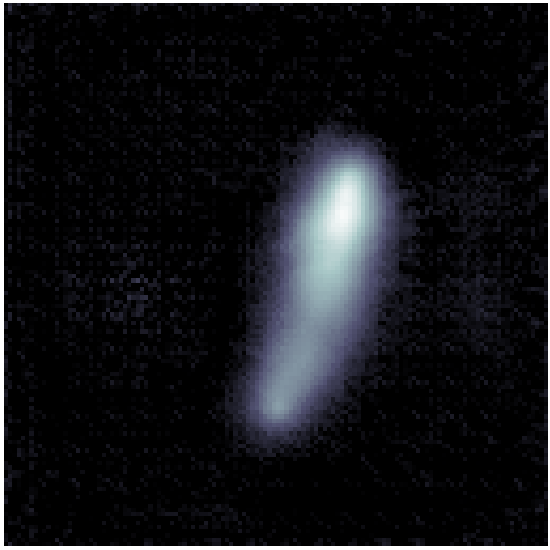
\includegraphics[width=2cm,height=2cm]{source_t2}};
  \end{scope}
  \node[scale=0.6, rotate=40] at (11.1, 1.4) {$\mathbf{\hat{s}}^{(t+1)}$};
  \begin{scope}[canvas is zy plane at x=11.6,transform shape]
	\node{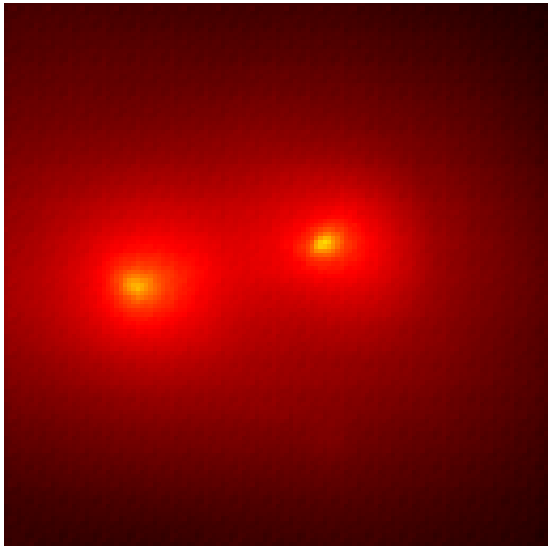
\includegraphics[width=2cm,height=2cm]{kappa_t2}};
  \end{scope}
  \node[scale=0.6, rotate=40] at (11.8, 1.4) {$\log\boldsymbol{\hat{\kappa}}^{(t+1)}$};

  \begin{scope}[canvas is yz plane at x=12.2,transform shape]
    \node{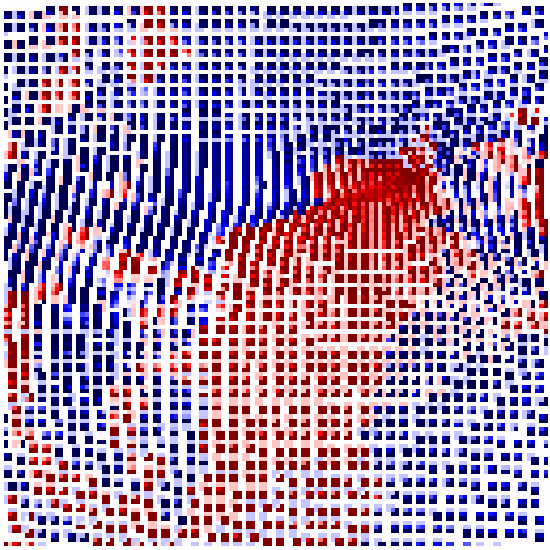
\includegraphics[width=2cm,height=2cm]{source_grad1}};
   %\node[rectangle, minimum size=2cm, fill=black!10, rotate=-90] at (0, 0) {$\grad_{\mathbf{y} \mid \mathbf{\hat{s}^{(t+1)}}}$};
   %\node[rectangle, minimum size=2cm, fill=black!10, rotate=-90] at (0, 0) {};
  \end{scope}
  \node[scale=0.6, rotate=40] at (12.4, 1.4) {$\grad_{\mathbf{y} \mid \mathbf{\hat{s}^{(t+1)}}}$};
  \begin{scope}[canvas is yz plane at x=12.8,transform shape]
    \node{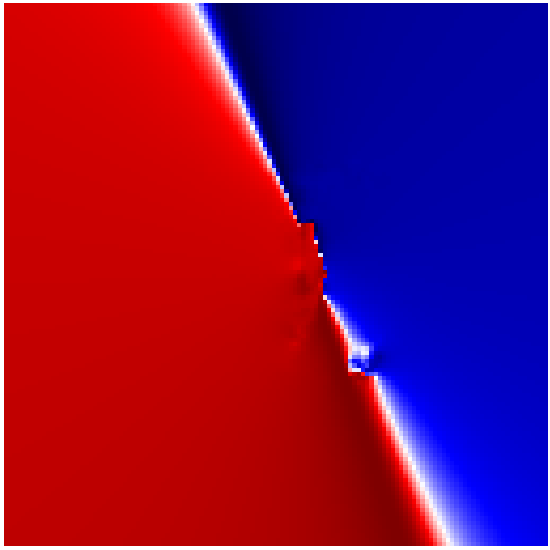
\includegraphics[width=2cm,height=2cm]{kappa_grad1}};
   %\node[rectangle, minimum size=2cm, fill=black!10, rotate=-90] at (0, 0) {$\grad_{\mathbf{y} \mid \boldsymbol{\hat{\kappa}^{(t+1)}}}$};
   %\node[rectangle, minimum size=2cm, fill=black!10, rotate=-90] at (0, 0) {};
  \end{scope}
  \node[scale=0.6, rotate=40] at (13, 1.4) {$\grad_{\mathbf{y} \mid \boldsymbol{\hat{\kappa}}^{(t+1)}}$};
  \begin{scope}[canvas is zy plane at x=13.4,transform shape]
	\node{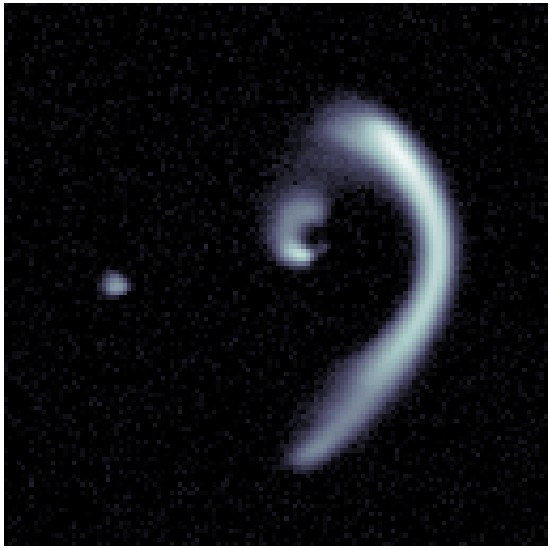
\includegraphics[width=2cm,height=2cm]{lens}};
  \end{scope}
        \node[scale=0.6, rotate=40] at (13.6, 1.4) {$\mathbf{y}$};

\node[rectangle, rounded corners, draw=black, fill=black!20, xscale=0.4, yscale=0.4, 
        minimum height=1cm, minimum width=2cm] at (11, -2.2) {Forward Model};

\draw[decorate,decoration={brace,amplitude=4pt,mirror},xshift=0pt,yshift=0pt,thick,color=darkgray] (10.6, -1.35) -- (11.7, -1.35);
\draw[-latex, color=darkgray] (11.15, -1.47) -- (11, -2);

\begin{scope}[canvas is zy plane at x=11,transform shape]
  \node (source) at (0, -4) {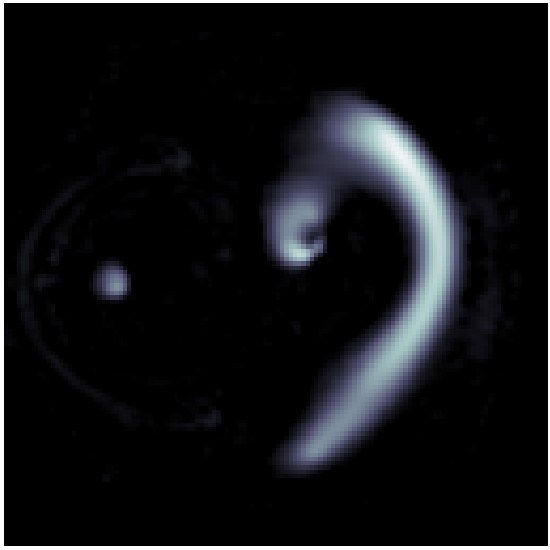
\includegraphics[width=1.5cm,height=1.5cm]{lens_t2}};
\end{scope}
\draw[-latex, color=darkgray] (11, -2.4) -- (11, -2.8);
\node[scale=0.6] at (11, -3) {$\mathbf{\hat{y}}^{(t+1)}$};


\node[rectangle, rounded corners, draw=black, fill=black!20, xscale=0.4, yscale=0.4, 
        minimum height=1cm, minimum width=2cm] (likelihood) at (12.75, -4) {Likelihood};
%\node[scale=0.6] (grads) at (12.2, -3.1) {$\grad_{\mathbf{y} \mid \mathbf{\hat{s}}^{(t+1)}}$};
%\node[scale=0.6]  (gradk) at (13.2, -3.1) {$\grad_{\mathbf{y} \mid \boldsymbol{ \hat{\kappa}}^{(t+1)}}$};
        
\node[rectangle, rounded corners, draw=black, fill=black!20, xscale=0.4, yscale=0.4, 
        minimum height=1cm, minimum width=2cm] (adam) at (12.75, -2.2) {Adam};
\draw[-latex, color=darkgray] (likelihood) to (adam);
%\draw[-latex, in=270, out=90, color=darkgray] (likelihood) to (grads);
%\draw[-latex, in=270, out=90, color=darkgray] (likelihood) to (gradk);
%\draw[-latex, in=270, out=90, color=darkgray] (grads) to (adam);
%\draw[-latex, in=270, out=90, color=darkgray] (gradk) to (adam);

\draw[decorate,decoration={brace,amplitude=4pt,mirror},xshift=0pt,yshift=0pt, thick, color=darkgray] (11.8, -1.35) -- (12.9, -1.35);
\draw[-latex,color=darkgray] (adam) to (12.34, -1.47);

\draw[-latex, color=darkgray] (11., -4) -- (12.33, -4);



\node[scale=0.6] at (-1, -1.7) {Legend};
\draw[thin] (-2, -1.8) -- (0, -1.8);

\pgfmathsetmacro{\cubex}{0.1}
\pgfmathsetmacro{\cubey}{0.2}
\pgfmathsetmacro{\cubez}{0.2}
\pgfmathsetmacro{\posx}{-1.8}
\pgfmathsetmacro{\posz}{0}
\pgfmathsetmacro{\posy}{-2.}
\draw[red,fill=pink] (\posx,\posy,\posz) -- ++(-\cubex,0,0) -- ++(0,-\cubey,0) -- ++(\cubex,0,0) -- cycle;
\draw[red,fill=pink] (\posx,\posy,\posz) -- ++(0,0,-\cubez) -- ++(0,-\cubey,0) -- ++(0,0,\cubez) -- cycle;
\draw[red,fill=pink] (\posx,\posy,\posz) -- ++(-\cubex,0,0) -- ++(0,0,-\cubez) -- ++(\cubex,0,0) -- cycle;

\node[scale=0.4, text width=7cm] at (-0.25, -2) {Input Convolution (Kernel size = $11\times 11$)};
\node[scale=0.4, text width=7cm] at (-0.25, -2.2) {Output Convolution (Kernel size = $1\times 1$)};

\pgfmathsetmacro{\cubex}{0.1}
\pgfmathsetmacro{\cubey}{0.2}
\pgfmathsetmacro{\cubez}{0.2}
\pgfmathsetmacro{\posx}{-1.8}
\pgfmathsetmacro{\posz}{0}
\pgfmathsetmacro{\posy}{-2.5}
\draw[brown,fill=orange] (\posx,\posy,\posz) -- ++(-\cubex,0,0) -- ++(0,-\cubey,0) -- ++(\cubex,0,0) -- cycle;
\draw[brown,fill=orange] (\posx,\posy,\posz) -- ++(0,0,-\cubez) -- ++(0,-\cubey,0) -- ++(0,0,\cubez) -- cycle;
\draw[brown,fill=orange] (\posx,\posy,\posz) -- ++(-\cubex,0,0) -- ++(0,0,-\cubez) -- ++(\cubex,0,0) -- cycle;

\node[scale=0.4, text width=6cm] at (-0.45, -2.55) {Transposed Convolution (Stride = $\frac{1}{2}$)};

\pgfmathsetmacro{\cubex}{0.1}
\pgfmathsetmacro{\cubey}{0.2}
\pgfmathsetmacro{\cubez}{0.2}
\pgfmathsetmacro{\posx}{-1.8}
\pgfmathsetmacro{\posz}{0}
\pgfmathsetmacro{\posy}{-3.}
\draw[blue,fill=cyan] (\posx,\posy,\posz) -- ++(-\cubex,0,0) -- ++(0,-\cubey,0) -- ++(\cubex,0,0) -- cycle;
\draw[blue,fill=cyan] (\posx,\posy,\posz) -- ++(0,0,-\cubez) -- ++(0,-\cubey,0) -- ++(0,0,\cubez) -- cycle;
\draw[blue,fill=cyan] (\posx,\posy,\posz) -- ++(-\cubex,0,0) -- ++(0,0,-\cubez) -- ++(\cubex,0,0) -- cycle;

\node[scale=0.4, text width=5.5cm] at (-0.55, -3.05) {Convolution (Stride = 2)};


\pgfmathsetmacro{\cubex}{0.1}
\pgfmathsetmacro{\cubey}{0.2}
\pgfmathsetmacro{\cubez}{0.2}
\pgfmathsetmacro{\posx}{-1.8}
\pgfmathsetmacro{\posz}{0}
\pgfmathsetmacro{\posy}{-3.5}
\draw[darkgray,fill=gray] (\posx,\posy,\posz) -- ++(-\cubex,0,0) -- ++(0,-\cubey,0) -- ++(\cubex,0,0) -- cycle;
\draw[darkgray,fill=gray] (\posx,\posy,\posz) -- ++(0,0,-\cubez) -- ++(0,-\cubey,0) -- ++(0,0,\cubez) -- cycle;
\draw[darkgray,fill=gray] (\posx,\posy,\posz) -- ++(-\cubex,0,0) -- ++(0,0,-\cubez) -- ++(\cubex,0,0) -- cycle;

\node[scale=0.4, text width=5.5cm] at (-0.55, -3.55) {Convolution (Stride = 1)};


\end{tikzpicture}

\end{document}
